%=============================================================================
% Tesis de Licenciatura: .....
%=============================================================================
   
%=============================================================================
%                                Preambulo Latex
%=============================================================================
\documentclass[oneside,letterpaper,10pt,spanish]{report}

%\usepackage[spanish]{babel} % division de silabas en español.
%\usepackage{ucs}
\usepackage[utf8]{inputenc} %%%Para poner acentos directamente

%\usepackage[T1]{fontenc}
%\usepackage[latin1]{inputenc}

%\usepackage{babel}
\setcounter{secnumdepth}{3} 
\setcounter{tocdepth}{3}  
\usepackage{makeidx}
\usepackage{graphics}  
\usepackage[boxed]{algorithm}
\usepackage{algorithmic}
\usepackage[dvips]{graphicx}
\usepackage{latexsym}
\usepackage{amssymb} 
\usepackage{amsthm}
\usepackage{url}
\usepackage{color}

\addtolength{\textwidth}{1cm} % Ancho del texto

% traducción de algunos nombres del paquete algorithm
\floatname{algorithm}{Algoritmo}
\renewcommand{\listalgorithmname}{Indice de algoritmos}

% Definiciones
\newtheorem{definition}{Definición}[section]

%Ejemplos
\newtheorem{ejemplo}{\normalfont \rule{0.2in}{0.11in}  {\rm Ejemplo }} [section]

%Casos de las reglas de reconstraccion
\newtheorem{caso}{\large {\rm Caso}}
 

%SUBCasos de las reglas de reconstraccion
\newtheorem{subcaso}{\large {\rm Caso}} [caso]

     
% Teoremas
\newtheorem{theorem}{Teorema}[section]

% Lemmas
\newtheorem{lema}{Lema}[section]

%%%%%%%%%%%%%%%% DEFINICIONES DE ALGUNOS COMANDOS Y AMBIENTES %%%%%%%%%%%%%%%

\newcounter{ruleAGcounter}
\newenvironment{AG}
{
 \setcounter{ruleAGcounter}{0} \begin{center} \begin{figure}[!hb]
 \rule{\textwidth}{.5pt} \footnotesize
}
{\normalsize \rule{\textwidth}{.5pt} \end{figure} \end{center}}
 
\newcommand{\newproduction}[2]{$p_\arabic{ruleAGcounter}$:
            \emph{#1} $\rightarrow$ \emph{#2}
            \addtocounter{ruleAGcounter}{1}\\}

%Por ahora al pedo esta lo que sigue
\newenvironment{micaso}[1][2] {\begin{caso} \textnormal{#1}} {\end{caso}}

%\newenvironment{proof}[1][Prueba]{}
 
\newcommand{\attribution}[1]{\hspace*{2cm}\emph{#1} \\} 

%Letra de los Estados
\newcommand{\letraEstado} [1] {\texttt{#1}}
%Letra de lso Diagramas de Clases
\newcommand{\letraDC} [1] {\texttt{#1}}
%Letra de las Funcionalidades
\newcommand{\letraFunc} [1] {\normalsize{#1}}
%Letra  del texto OR y AND
\newcommand{\letraORAND} [1] {\texttt{#1}}
%Color del texto
\newcommand{\textocolor} [1] {\textcolor{black}{#1}}
%Color del texto 2
\newcommand{\textocolorDos} [1] {\textcolor{black}{#1}}
%Color del texto 3
\newcommand{\textocolorTres} [1] {\textcolor{black}{#1}}


%letras de los elementos Ecore
\newcommand{\letraEcore} [1] {\texttt{#1}}
\newcommand{\letraRelaciones} [1] {\textbf{#1}}

\makeatother
\makeindex
 
%============================================================================

\pagestyle{empty} %get rid of header/footer for toc page
\begin{document}


\title{
UNIVERSIDAD NACIONAL DE RIO CUARTO\\
$\;$\\
$\;$\\
\small{Trabajo de tesis para la obtenci\'on del grado de Licenciatura en Ciencias de la Computaci\'on}
$\;$\\$\;$\\
\Large{\textbf{ T\'itulo .....}}
} 

\author{
                        Autores\\
                        Jaimez Jacinto \\
                        Pereyra Orcasitas Nicolás\\
                   ...@...\\ \\ \\
                 Director de Tesis: \emph{Mg. Marcela Daniele}\\ 
                 Co-Director de Tesis: \emph{Mg. Ariel Gonzalez}\\ 
}

\date{Rio Cuarto, Argentina\\ mes... 2016}

 
\maketitle
 

%Para dejar una página en blanco
\newpage
\mbox{}
\thispagestyle{empty} % para que no se numere esta página

%Incluye el abstact y los Agradecimientos.

%\begin{abstract}
\chapter*{Resumen}

\pagenumbering{roman} % para comenzar la numeracion de paginas en numeros romanos
\addcontentsline{toc}{chapter}{Resumen} % si queremos que aparezca en el índice

La tecnología de Web Service (WS) permite invocar aplicaciones externas, por ejemplo desde un motor de workflow y proporcionar beneficios significativos en el Workflow Management System (WFMS). Con el gran número de WS's que proporcionan una funcionalidad similar, es importante encontrar el mejor WS que cumpla con las necesidades del usuario, incluyendo tanto sus requisitos funcionales como los no funcionales. 
La descripción no funcional del Servicio requiere especificar en tiempo de ejecución los atributos de calidad que pueden influir en la elección de un WS ofrecido por un proveedor. En este sentido, es fundamental el uso de métricas para evaluar las características de calidad de los WS's (QoS) con el fin de filtrar los WS's conocidos y obtener el más adecuado.

El comportamiento dinámico de los WS’s en relación con el desarrollo de nuevos servicios y el constante cambio de los existentes requiere un proceso de evaluación continuo, que conduce a capturar información del WS con respecto a su calidad y rendimiento de evaluación conforme a lo solicitado por el workflow. En este trabajo se realiza un refinamiento del proceso de contrastación de WS ofrecidos por proveedores y solicitados por usuarios del workflow, se definen y usan métricas para evaluar los atributos de calidad de dichos servicios, y se propone una herramienta para automatizar este procedimiento de selección de aplicaciones externas al workflow

\emph{Palabras clave}: Web Service o WS, workflow, características de calidad o QoS

\thispagestyle{empty} % para que no se numere esta página
%\end{abstract}

\chapter*{Agradecimientos}
\addcontentsline{toc}{chapter}{Agradecimientos} % si queremos que aparezca en el índice

{\sl Queremos agradecer a todas las personas que han hecho posible la realización de esta tesis. A nuestros directores de tesis Marcela Daniele y Ariel Gonzalez, que han permitido llevar a un final exitoso este trabajo, por su asesoría, dedicación y sus valiosos aportes guiándonos sin ser directivas y mostrando en cada momento una inmejorable disposicón ante las dudas que durante la realización del trabajo nos surgieron, aportando siempre valiosas observaciones que tutelaron esta investigación.} {\sl A nuestras familias y amigos, por su incondicional apoyo durante este largo camino.}

{\sl Además, debemos retribuir con cordial gratitud tanto a la Universidad Nacional de Río Cuarto como a la Facultad de Ciencias Exactas, Físico-Químicas y Naturales, y en especial al Departamento de Computación, por permitirnos desarrollar nuestras formaciones individuales de grado con excelente material académico, pero sobre todo humano durante todos estos años.
}





%\end{flushright}

\listoffigures
\addcontentsline{toc}{chapter}{Lista de figuras} % para que aparezca en el indice de contenidos

%Las siguintes 3 lineas es para sacarle la numeracion de paginas al Indice
%\addtocontents{toc}{\protect\thispagestyle{empty}}
\tableofcontents %put toc in
%\cleardoublepage %start new page


%\pagestyle{fancy}
%\addtolength{\headwidth}{1cm} % Ancho del encabezado (fancy headers)
\renewcommand{\sectionmark}[1]{}
\renewcommand{\chaptermark}[1]{\markboth{#1}{}} % capíitulo en minísculas

%En la Introduccion se resetea el contador de paginas y el estilo de fuente de los numeros.

\chapter{Introducción}
\label{Introduccion}

.......


\pagenumbering{arabic} 
\setcounter{page}{1}


\section{Contribución}
\label{Contribucion del Trabajo}

La principal contribución de este trabajo es .... 

\section{Metas}
\label{Metas}

Puntualizando el propósito de este trabajo de investigación, se describe a continuación un conjunto de metas a alcanzar.
\begin{itemize}
 \item Relacionar y vincular los conceptos subyacentes....
 \item Mostrar que ...
 \item Presentar un mecanismo que permita  ....
\end{itemize}


\section{Organización del Trabajo}
\label{Organizacion del Trabajo}


El trabajo es organizado de la siguiente manera. 
En el capítulo \ref{Trabajos Relacionados}, hacemos mención de los trabajos relacionados con esta investigación. En el capítulo \ref{Nociones Preliminares}, introducimos los distintos formalismos, metodologías, estándares y 
teoría general que dan la base a la problemática planteada, tales como ....
En el capítulo \ref{}, presentamos el proceso de ....
Posteriormente, en el capítulo \ref{Ejemplo de Aplicacion} se exhibe un ejemplo de aplicación de la propuesta.
Finalmente, en el capítulo \ref{Conclusiones y Trabajos Futuros} se presentan las conclusiones y trabajos futuros.



\chapter{Trabajos Relacionados}
\label{Trabajos Relacionados}

....

\chapter{Nociones Preliminares}
\label{Nociones Preliminares}

En este capítulo se presentan los principales conceptos referentes a las áreas de base que dan soporte al trabajo, estas son: ...

En la sección \ref{}, hacemos una introducción a ....
En la sección \ref{Desarrollo Dirigido por Modelos} se describen brevemente los principios de MDD, en particular la propuesta concreta de la OMG conocida como MDA.
Y finalmente en la sección \ref{}, introducimos la base teórica de ...


\section{Servicios Web}
\label{Servicios Web}



\section{Desarrollo Dirigido por Modelos - MDD}
\label{Desarrollo Dirigido por Modelos}








\chapter{Selección de Servicios Web basada en MDD}
\label{Seleccion de Servicios Web basada en MDD} 








\chapter{Implementación ...}
\label{Implementacion}

...

\section{Análisis de los Lenguajes de Transformación de Modelos}\label{Analisis de los Lenguajes de Transformacion de Modelos}

En esta sección se analizan las propuestas existentes con el fin de fundamentar la elección del lenguaje utilizado en el actual trabajo.
El cuadro \ref{tabla:lenguajesdetransformacion} es una muestra de sólo algunos de una diversidad de lenguajes de transformación que se pueden
encontrar en la actualidad. Se muestra el gran número de propuestas existentes, que evidencia el gran interés que se ha despertado por este aspecto
del paradigma del desarrollo de software dirigido por modelos, así como la enorme actividad de investigación surgida alrededor del mismo.\\

\begin{table}[!hbt]
\begin{center}
\footnotesize
\begin{tabular}{| p{4cm}| p{8cm}|}
\hline
\textbf{Lenguaje/Implementación} & \textbf{Breve Descripción}\\
\hline
ATL (Atlas Transformation Language)  & Lenguaje de transformación de modelos y herramienta para Eclipse desarrollada por el Atlas Group (INRIA).\\
\hline
BOTL(Basic Object-Oriented Transformation Language) & Propuesta gráfica de la Universidad Técnica de München.\\
\hline
ETL (Epsilon Transformacion Language) &  Lenguaje definido sobre la plataforma Epsilon, plataforma desarrollada como un conjunto de plug-ins (editores, asistentes, pantallas de configuración, etc.) sobre Eclipse. Dicha plataforma presenta el lenguaje de metamodelado independiente Epsilon Object Language que se basa en OCL, y puede ser utilizado como lenguaje de gestión de modelos o como infraestructura a extender para producir nuevos lenguajes específicos de dominio, como el citado Epsilon Transformation Language (ETL). Además de ETL, Epsilon soporta a Epsilon Compari\-son Language (ECL) y a Epsilon Merging Language (EML), orientados a la comparación y composición de modelos, res\-pectivamente.\\
\hline
M2T (Model to Text project)  & Se focaliza en la generación de artefactos textuales a partir de modelos. Consta de un conjunto de herramientas desarrolladas para la plataforma Eclipse.\\
\hline
MTF (Model Transformation Framework) & Es un conjunto de herramientas desarrollado por IBM que permiten hacer comparaciones, comprobar la consistencia y ejecutar transformaciones entre modelos EMF.\\
\hline
MTL (Model Transformation Language) & Lenguaje de transformación de modelos y herramienta en Eclipse desarrollada por el grupo Triskell.\\
\hline 
QVT (Query/View/Transformation) & Especificación estándar de OMG. Está basado en MOF (Meta Object Facility) para lenguajes de transformación en MDA. 
Implementaciones: 
\begin{tabular}{p{2,5cm} p{4.7cm}}
QVT$-$Operational: & QVT Operacional de Borland\\
 & SmartQVT \\
 & Eclipse M2M\\
QVT-Core: & OptimalJ (Descontinuado)\\
 & QVT-Relations: \\
 & \hspace{0.5cm} MediniQVT\\
 & \hspace{0.5cm} Eclipse M2M Declarative QVT\\
 & \hspace{0.5cm} ModelMorf\\
\end{tabular}

\\  
\hline
 RubyTL & Lenguaje de transformación híbrido definido como un lenguaje específico del dominio embebido en el lenguaje de programación Ruby. Diseñado como un lenguaje extensible en el que un mecanismo de plugins permite añadir nuevas características al núcleo de características básicas.\\   

\hline
\end{tabular}
\caption{Lenguajes de transformación de modelos.}
\label{tabla:lenguajesdetransformacion}
\end{center}
\end{table}
\normalsize

Existe una variedad muy amplia de lenguajes de transformación, donde cada uno posee características deseables al igual que inconvenientes. Los lenguajes específicos del dominio (Domain Specific Language - DSL), como MT, ofrecen la ventaja de aprovechar todo el potencial del lenguaje \emph{host}, sumándole la expresividad y sofisticación del aparato transformacional. No obstante, esta característica también los hace poco compatible con otras herramientas que se basen en los estándares de la OMG (QVT, OCL, MOF, etc). Por otra parte, los lenguajes gráficos como UMLX son sumamente intuitivos pero a la vez limitados por la misma conformación de la simbología del lenguaje. Conjuntamente, la descripción de una transformación demasiada compleja puede resultar engorrosa para su utilización. Además, suelen incurrir en costos computacionales más elevados en comparación con lenguajes textuales, debido especialmente a que su representación es más compleja de procesar por su naturaleza gráfica. Los lenguajes de 
transformación M2T son bastante útiles para realizar implementaciones específicas de plataforma a partir de un modelo independiente de plataforma. Sin embargo, dejan de lado la transformación entre modelos, parte fundamental del desarrollo de software dirigido por modelos. En cualquier caso, actualmente muchas de las propuestas analizadas se encuentran en etapa de desarrollo, lo cual seguramente permitirá observar, en el futuro, mejoras en cada una de ellas.\\

QVT y los basados en éste, como por ejemplo ATL, tienen la ventaja de ceñirse a un estándar, lo cual los hace mas compatibles con otras tecnologías y comprensibles dada la formalidad de su especificación. Además, múltiples herramientas se han desarro\-llado que dan soporte a su implementación, entre ellas MEDINIQVT, la cual es una de las más robustas en la actualidad. Bajo las consideraciones mencionadas y otras comparativas efectuadas el lenguaje seleccionado para el actual trabajo es QVT.


\section{Lenguaje Query/View/Transformation Relations}
\label{Lenguaje Query/View/Transformation (QVT)}

La OMG ha definido el estándar Query/View/Transformation (QVT) \cite{QVT10} para utilizar en los procesos de desarrollo de software guiados por modelos. QVT consta de tres partes: consulta, vista y transformaciones. El componente de consultas de QVT toma como entrada un modelo y selecciona elementos específicos del mismo. Para la reso\-lución de las consultas y res\-tric\-ciones sobre los modelos, se propone el uso de una versión extendida de OCL 2.0 \cite{OCL20}. La parte de vista es una proyección realizada sobre un modelo y es creada mediante una transformación. Una vista puede verse como el resultado de una consulta sobre un modelo, ofreciendo como resultado un punto de vista de éste, restringiéndolo de acuerdo a alguna condición impuesta. 
En esta sección se presenta el componente de transformaciones de QVT que tiene como objetivo definir transformaciones. Estas transformaciones describen relaciones entre un metamodelo fuente \emph{F} y un metamodelo objetivo \emph{O}. Ambos metamodelos deben estar especificados con el estándar Meta-Object Facility (MOF) \cite{MOF11}. Una vez definida la transformación en QVT, ésta puede ejecutarse para obtener un modelo objetivo, que es una instancia del metamodelo \emph{O} a partir de un modelo fuente, el cual es una instancia del metamodelo \emph{F}.\\

La especificación de QVT 1.0 \cite{QVT10} tiene una naturaleza híbrida declarativa/im\-perativa, donde la parte declarativa se divide en una arquitectura de dos niveles
(ver figura \ref{fig:qvt}) constituida por un metamodelo y un lenguaje llamado \emph{Relations} que sigue un paradigma declarativo, el cual soporta 
concordancia de patrones (Pattern Matching) de objetos complejos y plantillas de creación de objetos, y un metamodelo y un lenguaje llamado \emph{Core}, 
definido usando mínimas extensiones de MOF y OCL.  En este trabajo se hace uso del lenguaje \emph{Relations} que permite especificar relaciones entre 
metamodelos MOF y de la herramienta para la definición de las transformaciones MediniQVT \cite{MED11}. 
Esta herra\-mienta implementa la especificación QVT/Relations en un poderoso motor QVT. Está diseñada para transformaciones de modelos permitiendo un 
rápido desarrollo, mantenimiento y particulari\-zación de reglas de transformación de procesos específicos. Su interfaz está basada en Eclipse y 
utiliza Eclipse Modeling Framework (EMF) \cite{EMF10} para la representación de los modelos. Además, posee un editor con asistente de código y un 
depurador de relaciones. MediniQVT exige que los metamodelos (y modelos) sean escritos en una variante simplificada del estándar MOF, llamada 
Ecore \cite{ECORE12}, el cual ha sido definido en el EMF.

\begin{figure}[!h] 
\begin{center}
 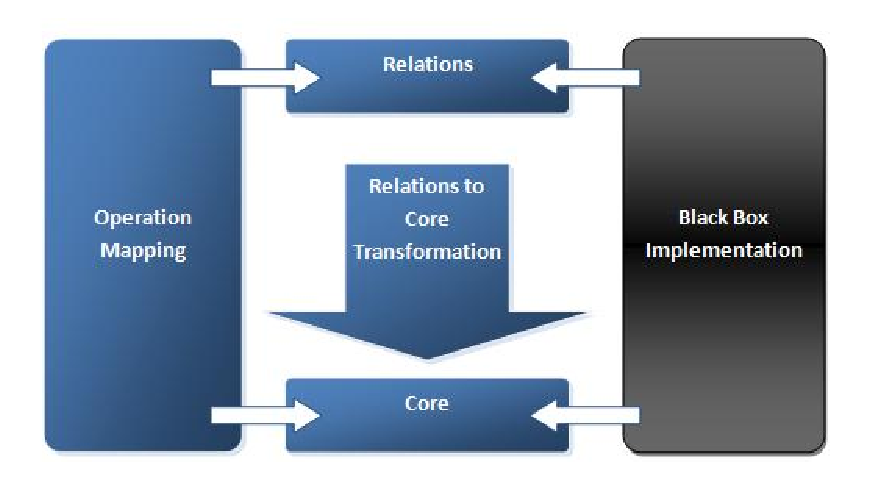
\includegraphics [scale=0.75]{imagenes/qvt.eps}
\end{center}
\caption{Arquitectura QVT.}
\label{fig:qvt}
\end{figure} 

\subsection*{Características de Eclipse Modeling Framework y Ecore}
\addcontentsline{toc}{subsection}{Características de Eclipse Modeling Framework y Ecore} % si queremos que aparezca en el índice

El lenguaje Ecore es el utilizado por el Eclipse Modeling Framework (EMF). Los metamodelos y modelos usados por EMF se representan con documentos XML. Existen herramientas que tratan automáticamente estos metamodelos y modelos. Por ejemplo, EMF ge\-ne\-ra código automáticamente para editores de modelos para un lenguaje de mode\-lado, definido con un metamodelo en Ecore. Otro ejemplo es el plug-in de Eclipse para transformar este tipo de modelos, con la definición de transformaciones QVT. Los metamodelos de Ecore son XML, sin embargo EMF posee un editor gráfico de modelos Ecore que facilita su creación.\\

Las características y elementos del lenguaje de modelado Ecore son los sigui\-entes: el elemento aglutinador (raíz) es el paquete \texttt{EPackage}, que contiene físicamente a sus elementos (especificación de
\texttt{containment}) y, a su vez, éstos pueden estar contenidos en otros paquetes. Hay una fábrica (\texttt{EFactory}) por paquete que permite la creación de los elementos del modelo. Las construcciones que describen a un conjunto de elementos (instancias) son clasificadores (\texttt{EClassifiers}): \texttt{EClass} y \texttt{EDataType}.\\

Ecore especifica las características de las clases (\texttt{EClass}), sus características estructurales (\texttt{EStructuralFeatures}), atributos (\texttt{EAttributes}), operaciones y relaciones (herencia, referencia (\texttt{EReference})). Las \texttt{EClasses} tienen superclases y están compuestas por características estructurales (\texttt{EStructuralFeatures}: \texttt{EReference} y \texttt{EAttribu\-te}). Tanto las \texttt{EReferences} como los \texttt{EAttributes} pueden estar dotados de multipli\-cidad.
Los \texttt{EDataTypes} modelan tipos básicos o indivisibles del modelo de datos, y los \texttt{EReferences} pueden estar contenidos o ser referencias (punteros).
Las \texttt{Operations} modelan operaciones de la interfaz (aunque no se provee implementación para ellas).
Todos los elementos heredan de \texttt{ENamedElement} (tienen nombre), y de \texttt{EModelElement} (elemento del modelo). Además, todo elemento del modelo puede te\-ner asociadas anotaciones (\texttt{EAnnotation}): pares nombre/valor para especificaciones extra (por ejemplo, restricciones OCL o cadenas de documentación). La figura \ref{fig:ECORE}, muestra la especificación del estándar Ecore.

\begin{figure}[H] 
\begin{center}
 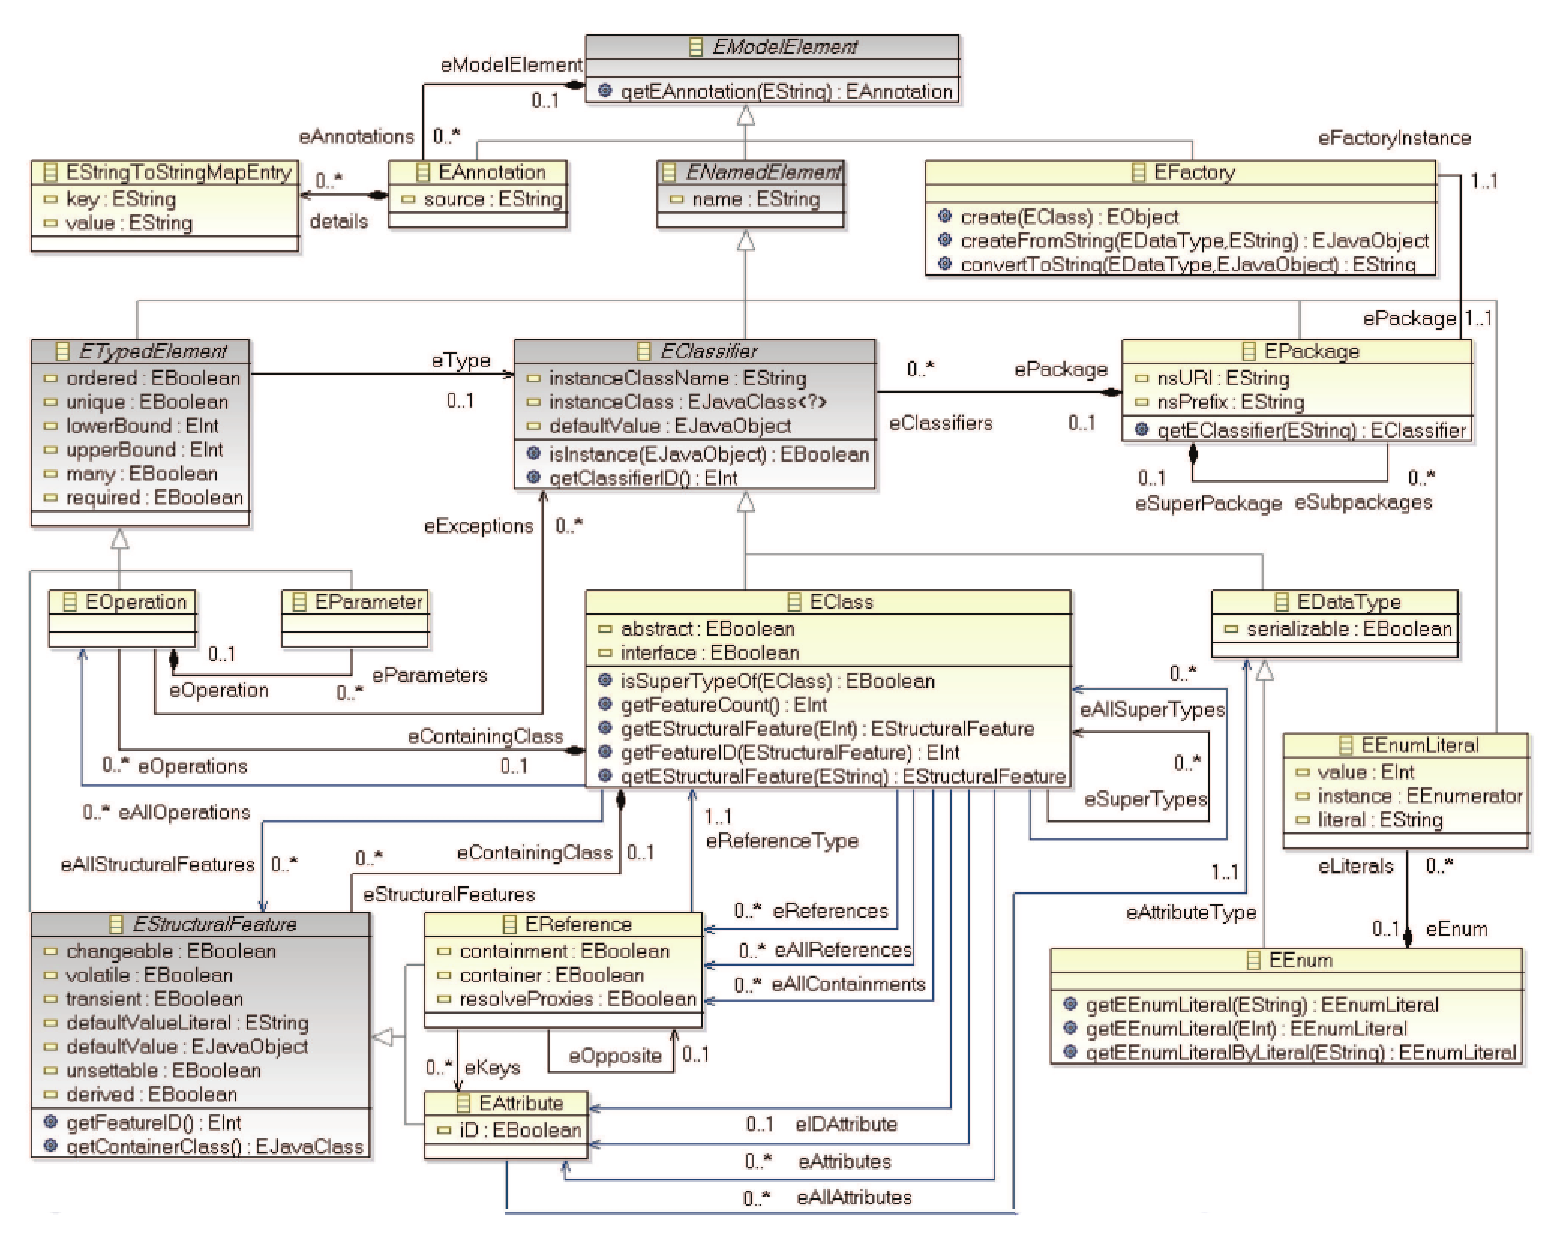
\includegraphics [width=135mm, height=120mm]{imagenes/ecore.eps}
\end{center}
\caption{Especificación del formato Ecore.}
\label{fig:ECORE}
\end{figure} 


\section{La Transformación}
\label{La Transformacion}

... hablar de la definiciones de las relaciones. Mostrar las partes de codigo mas relevantes de las relaciones.



\chapter{Ejemplo de Aplicación}
\label{Ejemplo de Aplicacion} 







\chapter{Conclusiones y Trabajos Futuros}
\label{Conclusiones y Trabajos Futuros}

....

%\include{Bibliography}

\bibliography{tesis}  
\bibliographystyle{IEEEtran}


\chapter*{Apéndices}
\label{Apendices}
\markboth{Apendices}{} % para que cambie el encabezado, si no, usaría el del último chapter{}
\addcontentsline{toc}{chapter}{Apéndices} % para que se añada en el indice

\appendix
\chapter{Especificación de la Transformación en Query/View/Transformation Relations}
\label{Especificacion de la Transformacion en QVT/Relations QVT}


%\section{Especificación de la Transformación en QVT/ Relations QVT}
%\label{Especificación de la Transformación en QVT/Relations QVT}
Código completo, en QVT Relation, de la transformación de máquinas de estados con elementos opcionales a máquinas de estados concretas.

\begin{verbatim}
-- Inicio de la Transformación 

\end{verbatim}


%Poner el codigo de la transformación por ejemplo

\printindex

\end{document}
